\documentclass[hyperref={pdfpagelabels=false}]{beamer}
\usepackage[utf8]{inputenc}
\usepackage[T1]{fontenc}
\usepackage{mathtools}

\usepackage{lmodern}
\usepackage{graphicx} 
\usepackage{multicol}
\usepackage{tikz}
\usepackage{framed}
\usepackage[mathscr]{euscript}
\usepackage{xcolor}
%\usepackage{cite}

\usepackage{mdframed}
\usepackage{algpseudocode}
%\usetheme{metropolis}
%\usecolortheme[named=cyan]{structure}

\definecolor{LHCblue}{RGB}{4, 114, 255}
\usecolortheme[named=LHCblue]{structure}
\usepackage[bars]{beamerthemetree}
\usetheme{Ilmenau}
\useoutertheme[subsection=true]{smoothbars}

\usepackage{enumerate}
\usepackage{mathrsfs}
\usepackage{amsmath,amssymb,amsthm}
\usepackage[ngerman]{babel}
\usepackage{color}


\title{Tensorstruktur der Zellmatrizen bei finiten Elementen }   
\author{Enes Witwit \\ Universität Heidelberg} 
\date{\today} 
\setbeamertemplate{navigation symbols}{}
%\usepackage{beamerthemeCambridgeUS}
\makeatother

\setbeamertemplate{headline}
{%
  \begin{beamercolorbox}[ht=3.5ex,dp=1.125ex,%
      leftskip=.3cm,rightskip=.3cm plus1fil]{section in head/foot}
    \usebeamerfont{section in head/foot}\usebeamercolor[fg]{section in head/foot}%
    \insertsectionhead
  \end{beamercolorbox}%
  \begin{beamercolorbox}[colsep=1.5pt]{middle separation line head}
  \end{beamercolorbox}
  \begin{beamercolorbox}[ht=2.5ex,dp=1.125ex,%
    leftskip=.3cm,rightskip=.3cm plus1fil]{subsection in head/foot}
    \usebeamerfont{subsection in head/foot}\insertsubsectionhead
  \end{beamercolorbox}%
  \begin{beamercolorbox}[colsep=1.5pt]{lower separation line head}
  \end{beamercolorbox}
}

\setbeamertemplate{footline}
{%
  \leavevmode%
  \hbox{\begin{beamercolorbox}[wd=.5\paperwidth,ht=2.5ex,dp=1.125ex,leftskip=.3cm,rightskip=.3cm]{author in head/foot}%
      \usebeamerfont{author in head/foot}\insertshortauthor
  \end{beamercolorbox}%
  \begin{beamercolorbox}[wd=.5\paperwidth,ht=2.5ex,dp=1.125ex,leftskip=.3cm,rightskip=.3cm plus1fil]{title in head/foot}%
    \usebeamerfont{author in head/foot}\insertshorttitle\hfill\insertpagenumber/\inserttotalframenumber
  \end{beamercolorbox}}%
  \vskip0pt%
}
\setbeamertemplate{footline}[frame number]{}

\makeatletter
\beamersetuncovermixins{\opaqueness<1>{25}}{\opaqueness<2->{15}}

\setbeamercovered{invisible}


\begin{document}
%Titlepage
\begin{frame}[noframenumbering, plain]
\titlepage
\end{frame} 


%Contents
\begin{frame}[noframenumbering, plain]
\frametitle{Contents}
\setcounter{tocdepth}{1}
\small{ \tableofcontents}
\end{frame}

% Introduction
\section{Einleitung} 
\begin{frame}[noframenumbering, plain]
\small{\tableofcontents[currentsection]}
\end{frame}
\begin{frame}
\frametitle{Hochleistungsrechnen}
\begin{framed}
\center{\textbf{Ziel} Löse ein sehr komplexes Problem.}
\end{framed} 
\center{ \textbf{Lösungsansatz} }
Teile das komplexe Problem auf in Subprobleme (Parallelisierung).
\end{frame}


\begin{frame}
\frametitle{Initial-Problem}
\begin{framed}
\begin{equation*}
v = A(u)
\end{equation*}
A, möglicherweise nichtlinearer, finite Elemente Operator, der Vektor u als Input nimmt.
\end{framed}
Probleme 
\begin{itemize}
\item $A$ wird unter Umständen sehr groß $\rightarrow$ Speicherplatz.
\item $A$ liegt nicht mehr im Cache $\rightarrow$ Abrufen der Elemente von $A$ zeitintesiv. 
\item Berechnung des Matrix-Vektor-Produkts komplex
\end{itemize}
\end{frame}

\begin{frame}
\frametitle{Divide and Conquer}
Nach \cite{Kronbichler} können wir die Ursprungsgleichung umformen zu
\begin{equation*}
v = A(u) = \sum\limits_{k=1}^{n_{cells}} P_k^T A_k P_k u \, .
\end{equation*}
$P_k$ kümmert sich um die Einordnug der lokalen Freiheitsgrade in die globalen Freiheitsgrade.
\begin{framed}
\begin{align*}
v_k &= A_k u_k \\
A_k^{-1} v_k &= u_k
\end{align*}
\end{framed}
\end{frame}

\begin{frame}
\frametitle{Inverse/Pseudoinverse}
\begin{enumerate}
\item Tensorstruktr und Summenfaktorisierung.
\item Singulärwertzerlegung höherer Ordnung (HOSVD).
\end{enumerate}

\end{frame}


% Theorie
\section{Theorie}
\begin{frame}[noframenumbering, plain]
\small{\tableofcontents[currentsection]}
\end{frame}
\begin{frame}
\frametitle{Higher Order Singular Value Decomposition}
\begin{framed}
Defintion \\

\end{Definition}

\end{frame}

% Pseudoinverse
\section{Pseudoinverse}
\begin{frame}[noframenumbering, plain]
\small{\tableofcontents[currentsection]}
\end{frame}
\subsection{Tensorstruktur}

% Definition Masse und Laplace Matrix
\begin{frame}

\begin{framed}
\textbf{Lokale Massenmatrix}
\begin{equation*} \label{eq:mass}
M_{ik} = \int\limits_{T} \varphi_i (\bold{x}) \, \varphi_j (\bold{x}) \, d\bold{x}
\end{equation*}

\textbf{Elementsteifigkeitsmatrix der Laplace Bilinearform}
\begin{equation*}
V_{ij} = \int\limits_{T} \nabla \varphi_i(\bold{x}) \, \nabla \varphi_j(\bold{x})  d \bold{x}
\end{equation*}
\end{framed}

\begin{itemize}
\item $T$ sei die Referenzzelle für Rechtecke
\item $\varphi_i(\bold{x})$ sei eine zweidimensionale reelle Basisfunktion des diskreten Raumes $V_n$ mit $\bold{x}=(x,y)$ .
\end{itemize}

\end{frame}



% Tensorstruktur der Ansatzfunktionen
\begin{frame}
\frametitle{Tensorstruktur der Ansatzfunktionen}

\begin{equation*} \label{eq:tensor}
\varphi^{2D}_i(\bold{x})=\varphi^{2D}_{i_1+(N+1)i_2}(x,y)=\varphi^{1D}_{i_1}(x)\varphi^{1D}_{i_2}(y),
\end{equation*}

\begin{figure}[ht] 
	\centering
  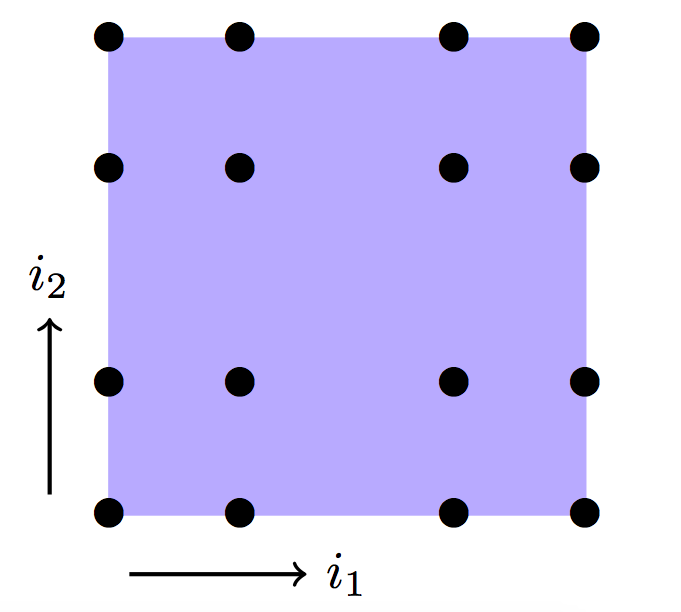
\includegraphics[width=0.3\textwidth]{lexi.png}
	\caption{ \cite[3]{Teachlet}}
	\label{fig:lexi}
\end{figure}

\end{frame}

\begin{frame}
\frametitle{Tensorstruktur der Massenmatrix}
Es seien $\bold{x}_q=(x_{q1},x_{q2})$ die Stützstellen und $\bold{w}_q=w_{q1}w_{q2}$ die Gewichte der Gauss Quadratur.
\begin{equation*} \label{eq:massapprox}
\begin{aligned}
M_{ij} &= \int\limits_{T} \varphi_i (\bold{x}) \, \varphi_j (\bold{x}) \, d\bold{x} \\ \pause
&\approx  \sum\limits_{q=1}^Q \bold{w}_q \, \, \varphi_i (\bold{x}_q) \, \varphi_j (\bold{x}_q) \\ \pause
&= \sum\limits_{q_1=1}^{Q_{1D}} \sum\limits_{q_2=1}^{Q_{1D}} \varphi_{i_1}(x_{q1}) \varphi_{i_2}(x_{q2}) \varphi_{j_1}(x_{q1}) \varphi_{j_2}(x_{q2}) \, w_{q1} w_{q2} \\ 
&= \sum\limits_{q_1=1}^{Q_{1D}} w_{q1} \varphi_{i_1}(x_{q1}) \varphi_{j_1}(x_{q1}) \sum\limits_{q_2=1}^{Q_{1D}} w_{q2} \varphi_{i_2}(x_{q2}) \varphi_{j_2}(x_{q2}) \, . 
\end{aligned}
\end{equation*}
\end{frame}

\begin{frame}
\textbf{Definiere} \\
\begin{itemize}
\item Es sei $\mathcal{N}$ eine Matrix mit $\mathcal{N}_{iq}=\varphi_i(\bold{x}_q)$.
\item Es sei $\mathcal{W}$ eine Matrix mit $\mathcal{W}_{ii}=\bold{w}_i$, sonst Nullen.
\end{itemize}
Dann können wir die Massenmatrix schreiben als
\begin{equation*}
M = \underbrace{\mathcal{N} \mathcal{W}}_{:=\mathcal{W}_N} \mathcal{N}^T. = \mathcal{W}_N \mathcal{N}^T
\end{equation*}
\pause
\textbf{Nutze Tensorstruktur der Ansatzfunktionen}
\begin{equation*}
\begin{aligned}
\mathcal{N} &= \mathcal{N}^{1D} \otimes \mathcal{N}^{1D} \\
\mathcal{W}_N &= \mathcal{W}_N^{1D} \otimes \mathcal{W}_N^{1D}
\end{aligned}
\end{equation*}
\end{frame}

\begin{frame}
\frametitle{Tensorstruktur der Massenmatrix}
\begin{framed}
\begin{equation*}
\begin{aligned}
M &= \mathcal{W}_N \mathcal{N}^T \\
&= (\mathcal{W}_N^{1D} \otimes \mathcal{W}_N^{1D})(\mathcal{N}^{1D} \otimes \mathcal{N}^{1D})^T \\
&= (\mathcal{W}_N^{1D} \otimes \mathcal{W}_N^{1D})((\mathcal{N}^{1D})^T \otimes (\mathcal{N}^{1D})^T) \\
&= (\mathcal{W}_N^{1D} (\mathcal{N}^{1D})^T) \otimes  (\mathcal{W}_N^{1D} (\mathcal{N}^{1D})^T) 
\end{aligned}
\end{equation*}
\end{framed}
\end{frame}

\begin{frame}
\frametitle{Pseudoinverse der Massenmatrix}
\begin{equation*}
\begin{aligned}
M^+ & = [(\mathcal{W}_N^{1D} (\mathcal{N}^{1D})^T) \otimes  (\mathcal{W}_N^{1D} (\mathcal{N}^{1D})^T)]^+ \\ &= (\mathcal{W}_N^{1D} (\mathcal{N}^{1D})^T)^+ \otimes  (\mathcal{W}_N^{1D} (\mathcal{N}^{1D})^T)^+ 
\end{aligned}
\end{equation*}
\end{frame}





\begin{frame}
\frametitle{Tensorstruktur der Laplace Bilinearform}
\begin{equation*}
\begin{aligned}
V_{ij} &= \int\limits_{T} \nabla \varphi_i(\bold{x}) \, \nabla \varphi_j(\bold{x})  d \bold{x} \\ 
&= \int\limits_{T}( \partial_{x_1}  \varphi_i(\bold{x})  \partial_{x_1} \varphi_j(\bold{x})) + ( \partial_{x_2} \varphi_i(\bold{x})  \partial_{x_2} \varphi_j(\bold{x})) \, d\bold{x} \\
&= \int\limits_{T}( \partial_{x_1}  \varphi_i(\bold{x})  \partial_{x_1} \varphi_j(\bold{x})) + ( \partial_{x_2} \varphi_i(\bold{x})  \partial_{x_2} \varphi_j(\bold{x})) \, d\bold{x} \\ &= \int\limits_{T} \partial_{x_1}  \varphi_i(\bold{x})  \partial_{x_1} \varphi_j(\bold{x}) d\bold{x} + \int\limits_{T}  \partial_{x_2} \varphi_i(\bold{x})  \partial_{x_2} \varphi_j(\bold{x}) \, d\bold{x} \\
&= \underbrace{\sum\limits_{q=1}^{(N+1)^2} \bold{w}_q \partial_{x_1}  \varphi_i(\bold{x}_q)  \partial_{x_1} \varphi_j (\bold{x}_q)}_{K^1} + \underbrace{\sum\limits_{q=1}^{(N+1)^2} \bold{w}_q  \partial_{x_2} \varphi_i(\bold{x}_q)  \partial_{x_2} \varphi_j(\bold{x}_q)}_{K^2} \, 
\end{aligned}
\end{equation*}
\end{frame}

\begin{frame}
\begin{equation*}
\begin{aligned}
K_{ij}^1 &=\sum\limits_{q=1}^{(N+1)^2} \bold{w}_q \partial_{x_1}  \varphi_i(\bold{x}_q)  \partial_{x_1} \varphi_j (\bold{x}_q) \\ &= \sum\limits_{q_1=1}^{N} \sum\limits_{q_2=1}^{N} w_{q1}w_{q2} \partial_{x_1}  \varphi_{i1}(x_{q1})\varphi_{i2}(x_{q2})  \partial_{x_1} \varphi_{j1} (x_{q1})\varphi_{j2} (x_{q2}) \\
&=  \sum\limits_{q_1=1}^{N} \sum\limits_{q_2=1}^{N} w_{q1}w_{q2} \varphi'_{i1}(x_{q1})\varphi_{i2}(x_{q2})  \varphi'_{j1} (x_{q1})\varphi_{j2} (x_{q2}) \\ 
&= \sum\limits_{q_1=1}^{N} w_{q1} \varphi'_{i1}(x_{q1}) \varphi'_{j1} (x_{q1}) \sum\limits_{q_2=1}^{N} w_{q2} \varphi_{i2}(x_{q2})  \varphi_{j2} (x_{q2}) 
\end{aligned}
\end{equation*}
\end{frame}

\begin{frame}
\textbf{Definiere}
\begin{itemize}
\item Es sei $\widehat{\mathcal{N}}^{1D}$ eine Matrix mit $\widehat{\mathcal{N}}^{1D}_{ik}=\varphi'^{1D}_i(x_k)$
\item Dementsprechend ist $\widehat{\mathcal{W}}^{1D}_N$ eine Matrix, die aufgebaut ist wie $\mathcal{W}^{1D}_N$, mit dem Unterschied, dass sie die Evaluationen der ersten Ableitungen der Ansatzfunktionen beinhaltet.
\end{itemize}
\pause
\textbf{Dann} können wir $K_1,K_2$ schreiben als
\begin{align*}
K_1 &= (\widehat{\mathcal{W}}_N^{1D} (\widehat{\mathcal{N}}^{1D})^T) \otimes (\mathcal{W}_N^{1D}(\mathcal{N}^{1D})^T) \\
K_2 &= (\mathcal{W}_N^{1D} (\mathcal{N}^{1D})^T) \otimes (\widehat{\mathcal{W}}_N^{1D} (\widehat{\mathcal{N}}^{1D})^T)
\end{align*}
\begin{framed}
\begin{equation*}
V =\widehat{\mathcal{W}}_N \widehat{\mathcal{N}}^T \otimes \mathcal{W}_N \mathcal{N}^{T} + \mathcal{W}_N \mathcal{N}^{T}\otimes \widehat{\mathcal{W}}_N \widehat{\mathcal{N}}^T.
\end{equation*}
\end{framed}
\end{frame}

\begin{frame}
\frametitle{Problem bei Laplace}
\textbf{Problem } Die Addition in der Tensorstruktur macht unseren ersten Ansatz hinfällig. \\
\textbf{Idee } Vereinfache die Form durch geeignete Basiswahl und dann sehen wir weiter. Wir wählen geeignete Basis, sodass $ \, \mathcal{W}_N \mathcal{N}^{T} = I_n \, $.

Folgende Basispolynome bieten sich an:
\begin{framed}
\begin{equation*}
\varphi^{1D}_i (x_k) = \dfrac{1}{ \sqrt{w_i} } l_i (x_k) = 
\begin{cases}
\dfrac{1}{ \sqrt{w_i} } \, \text{ , wenn } i=k  \\
0  \, \, \, \, \, \, \, \, \, \, \, \text{ , sonst. }
\end{cases}
\end{equation*}
Die Funktion $l_i(x_k)$ bezeichnet das $i-te$ Lagrange Polynom.
\end{framed}
\end{frame}


% Effiziente Berechnung
\section{Effiziente Berechnung}
\begin{frame}[noframenumbering, plain]
\small{\tableofcontents[currentsection]}
\end{frame}
%\input{processing.tex}



\section*{Literatur}
\begin{frame}
\frametitle{Bibliography}
\begin{itemize}
\item Example

\end{itemize}
\end{frame}

\begin{frame}
\bibliographystyle{alpha}
\bibliography{literatur}
\end{frame}



\end{document}